\chapterbackmatter{Solutions to Supplementary Exercises}

\begin{enumerate}
\SupplementarySolution{1}{Symmetries, Currents, Charges, and Lorentz Boosts}
\begin{enumerate}
\item
A continuous symmetry is a differentiable family of field
transformations
\[
 \phi(x)\longmapsto\phi(x)+\epsilon\,\Delta\phi(x)+O(\epsilon^2)
\]
under which the action is unchanged, possibly up to a boundary term.
A conserved current is a local vector \(j^\mu\) satisfying
\(\partial_\mu j^\mu=0\) on the equations of motion.  Its charge is
\[
 Q(t)=\int d^3x\,j^0(t,\mathbf x).
\]
Current conservation implies
\[
 \dot Q=-\int d^3x\,\boldsymbol\nabla\cdot\mathbf j
       =-\oint_{S_\infty}d\mathbf S\cdot\mathbf j,
\]
so \(Q\) is conserved when the flux at spatial infinity vanishes.

Noether's first theorem takes a differentiable action symmetry to an
on-shell conserved current; it assumes the variational equations and
keeps track of any boundary term in the action variation.  A conserved
local current gives a conserved charge only with suitable boundary
conditions.  Conversely, a charge gives a symmetry when it is a
well-defined canonical generator, for example
\(\delta\phi=i\epsilon[Q,\phi]\), and conservation is equivalent to
\([Q,H]=0\) when the charge has no explicit time dependence.  An inverse
Noether statement from a current to a local variational symmetry also
requires a regular local action and is understood modulo identically
conserved improvement currents.  These qualifications are why none of
the three implications is purely formal.
\item
For translations, the scalar energy--momentum tensor in the volume's
convention is
\[
 T^{\rho\sigma}
 =(\partial^\rho\phi)(\partial^\sigma\phi)
  +\eta^{\rho\sigma}\mathcal L
 =(\partial^\rho\phi)(\partial^\sigma\phi)
  -\eta^{\rho\sigma}\left[
    \frac12\partial_\mu\phi\,\partial^\mu\phi+V(\phi)\right].
\]
The field equation is \(\Box\phi=V'(\phi)\).  Direct differentiation
then gives
\[
 \partial_\rho T^{\rho\sigma}
 =(\Box\phi-V')\partial^\sigma\phi=0.
\]
For each fixed \(\sigma\), \(T^{\rho\sigma}\) is a conserved current.
The corresponding four charges are
\[
 P^\sigma=\int d^3x\,T^{0\sigma},
\]
namely the energy and the three components of momentum, with the
index-position signs fixed as in Section 7.3.
\item
For a scalar,
\[
 \delta\phi
 =-\frac12\omega_{\rho\sigma}
  (x^\rho\partial^\sigma-x^\sigma\partial^\rho)\phi.
\]
Noether's theorem therefore gives the six Lorentz currents
\[
 M^{\mu\rho\sigma}
 =x^\rho T^{\mu\sigma}-x^\sigma T^{\mu\rho}.
\]
Equivalently, differentiating and using symmetry of the scalar tensor,
\[
\begin{split}
 \partial_\mu M^{\mu\rho\sigma}
 &=T^{\rho\sigma}-T^{\sigma\rho}
   +x^\rho\partial_\mu T^{\mu\sigma}
   -x^\sigma\partial_\mu T^{\mu\rho}=0.
\end{split}
\]
\item
Let
\[
 X^i(t)=\int d^3x\,x^iT^{00}.
\]
Stress-tensor conservation and vanishing surface terms give
\[
\begin{split}
 \dot X^i
 &=-\int d^3x\,x^i\partial_jT^{j0}
   =\int d^3x\,T^{i0}
   =\int d^3x\,T^{0i}=P^i.
\end{split}
\]
Thus the vector defined in the problem is
\(V^i=\dot X^i=P^i\).  Since the translation charge is conserved,
\(\dot V^i=\dot P^i=0\).
\end{enumerate}

\SupplementarySolution{2}{The Maxwell Stress Tensor and Metric Response}
\begin{enumerate}
\item
The variation of the field strength is
\[
 \delta F_{\mu\nu}
 =\partial_\mu\delta A_\nu-\partial_\nu\delta A_\mu.
\]
Using antisymmetry and integrating by parts,
\[
 \delta S
 =\int d^4x\,
 \left(\partial_\mu F^{\mu\nu}-j^\nu\right)\delta A_\nu,
\]
so
\[
 \partial_\mu F^{\mu\nu}=j^\nu.
\]
The \(\nu=0\) equation is
\[
 \boldsymbol\nabla\cdot\mathbf E=j^0,
\]
and the spatial equations are
\[
 \boldsymbol\nabla\times\mathbf B-\partial_t\mathbf E
 =\mathbf j.
\]
The remaining two Maxwell equations follow instead from
\(\partial_{[\lambda}F_{\mu\nu]}=0\):
\[
 \boldsymbol\nabla\cdot\mathbf B=0,\qquad
 \boldsymbol\nabla\times\mathbf E+\partial_t\mathbf B=0.
\]
This makes explicit the terminology correction recorded in the prompt.
\item
In the energy--momentum convention of this volume, the canonical tensor
is
\[
 T_{\rm can}^{\mu\nu}
 =F^{\mu\lambda}\partial^\nu A_\lambda
  -\frac14\eta^{\mu\nu}F_{\rho\sigma}F^{\rho\sigma}.
\]
The explicit \(A_\lambda\) makes it gauge dependent, and
\(T_{\rm can}^{\mu\nu}\ne T_{\rm can}^{\nu\mu}\).  In the source's
opposite canonical-tensor convention the stated improvement is
\(+\partial_\lambda(F^{\mu\lambda}A^\nu)\); after translating to the
volume's convention it is
\[
 \widetilde T^{\mu\nu}
 =T_{\rm can}^{\mu\nu}
 -\partial_\lambda(F^{\mu\lambda}A^\nu).
\]
For \(j^\mu=0\),
\[
 \partial_\lambda(F^{\mu\lambda}A^\nu)
 =F^{\mu\lambda}\partial_\lambda A^\nu,
\]
and hence
\[
 \widetilde T^{\mu\nu}
 =F^{\mu\lambda}F^\nu{}_\lambda
  -\frac14\eta^{\mu\nu}F_{\rho\sigma}F^{\rho\sigma}.
\]
This expression is symmetric and contains only \(F\), so it is gauge
invariant.  Antisymmetry of the first two indices of the improvement
superpotential makes its double divergence vanish identically; its
spatial integral is a surface term, so the total four-momentum is
unchanged.

Using
\(F_{\rho\sigma}F^{\rho\sigma}
=2(\mathbf B^2-\mathbf E^2)\), one obtains
\[
 \widetilde T^{00}
 =\frac12(\mathbf E^2+\mathbf B^2),
\qquad
 \widetilde T^{0i}=(\mathbf E\times\mathbf B)^i.
\]
\item
At \(j^\mu=0\), vary
\[
 S[A,g]=-\frac14\int d^4x\,\sqrt{|g|}\,
 F_{\mu\nu}F_{\rho\sigma}g^{\mu\rho}g^{\nu\sigma}.
\]
The determinant variation in inverse-metric variables is
\[
 \delta\sqrt{|g|}
 =-\frac12\sqrt{|g|}\,g_{\mu\nu}\delta g^{\mu\nu}.
\]
The two inverse metrics in the Maxwell term give equal contributions.
After symmetrizing the free metric indices,
\[
 \delta S
 =-\frac12\int d^4x\,\sqrt{|g|}
 \left[
 F_{\mu\rho}F_\nu{}^\rho
 -\frac14g_{\mu\nu}F_{\rho\sigma}F^{\rho\sigma}
 \right]\delta g^{\mu\nu}.
\]
Therefore the mostly-plus response definition in the prompt yields
\[
 T^{(g)}_{\mu\nu}
 =F_{\mu\rho}F_\nu{}^\rho
  -\frac14g_{\mu\nu}F_{\rho\sigma}F^{\rho\sigma}.
\]
Raising both indices and taking \(g_{\mu\nu}=\eta_{\mu\nu}\) reproduces
the improved tensor in part (b).  Symmetry follows because the
functional derivative is with respect to the symmetric metric, and
gauge invariance follows because the metric-coupled action depends on
\(A_\mu\) only through \(F_{\mu\nu}\) when \(j^\mu=0\).
\end{enumerate}

\SupplementarySolution{3}{A Complex Scalar Field}
\begin{enumerate}
\item
Under \(x\mapsto x'=\Lambda x\), a scalar obeys
\(\phi'(x')=\phi(x)\), and similarly for \(\phi^\dagger\).
The measure \(d^4x\), the contraction
\(\partial_\mu\phi^\dagger\partial^\mu\phi\), and
\(\phi^\dagger\phi\) are Lorentz invariant, so \(S'=S\).
Independent variation of \(\phi\) and \(\phi^\dagger\) gives
\[
 \Box\phi-V'(\phi^\dagger\phi)\phi=0,\qquad
 \Box\phi^\dagger-V'(\phi^\dagger\phi)\phi^\dagger=0.
\]
\item
The momenta and Hamiltonian density are
\[
 \pi=\dot\phi^\dagger,\qquad \pi^\dagger=\dot\phi,\qquad
 \mathcal H=\pi\pi^\dagger+\nabla\phi^\dagger\cdot\nabla\phi
 +V(\phi^\dagger\phi).
\]
Hamilton's equations reproduce the two equations in part 1.
\item
Under
\(\delta\phi=i\epsilon\phi\) and
\(\delta\phi^\dagger=-i\epsilon\phi^\dagger\), the chapter's Noether
normalization gives
\[
 j^\mu=i\left[\phi^\dagger\partial^\mu\phi
              -(\partial^\mu\phi^\dagger)\phi\right].
\]
The charge is therefore
\[
 Q=\int d^3x\,j^0
 =i\int d^3x\left(
 \dot\phi^\dagger\phi-\phi^\dagger\dot\phi\right).
\]
\item
Direct differentiation cancels the terms bilinear in first
derivatives:
\[
 \partial_\mu j^\mu
 =i\left[\phi^\dagger\Box\phi
         -(\Box\phi^\dagger)\phi\right].
\]
Using the two equations from part (a), both terms become
\(iV'(\phi^\dagger\phi)\phi^\dagger\phi\) with opposite signs.
Thus \(\partial_\mu j^\mu=0\), as required.
\end{enumerate}

\SupplementarySolution{4}{The Energy--Momentum Tensor of a Complex Scalar}
\begin{enumerate}
\item
The scalar transformation law gives
\(\phi'(x)=\phi(x-a)\) and
\(\phi'^\dagger(x)=\phi^\dagger(x-a)\).  Hence
\[
\begin{split}
 S'&=\int d^4x\left[
 -\partial_\mu\phi^\dagger(x-a)\partial^\mu\phi(x-a)
 -V\!\left(\phi^\dagger(x-a)\phi(x-a)\right)\right]\\
 &=S
\end{split}
\]
after the translation \(y=x-a\), whose Jacobian is one.
\item
Infinitesimally,
\[
 \delta\phi=-a^\rho\partial_\rho\phi,\qquad
 \delta\phi^\dagger=-a^\rho\partial_\rho\phi^\dagger,\qquad
 \delta\mathcal L=-a^\rho\partial_\rho\mathcal L.
\]
Noether's theorem, with the coefficient of each independent
\(a^\rho\) extracted, gives the symmetric tensor
\[
 T^{\mu\nu}
 =(\partial^\mu\phi^\dagger)\partial^\nu\phi
 +(\partial^\nu\phi^\dagger)\partial^\mu\phi
 +\eta^{\mu\nu}\mathcal L .
\]
For every fixed \(\nu\), \(T^{\mu\nu}\) is the current associated with
translation in that direction.
\item
Because \(\partial^0=-\partial_0\) and \(\eta^{00}=-1\),
\[
 T^{00}
 =\dot\phi^\dagger\dot\phi
  +\boldsymbol\nabla\phi^\dagger\cdot\boldsymbol\nabla\phi
  +V(\phi^\dagger\phi).
\]
Thus
\[
 H=\int d^3x\left[
 \dot\phi^\dagger\dot\phi
 +\boldsymbol\nabla\phi^\dagger\cdot\boldsymbol\nabla\phi
 +V(\phi^\dagger\phi)\right],
\]
which agrees with the Legendre transform in S.7.3(b), since
\(\pi=\dot\phi^\dagger\) and
\(\pi^\dagger=\dot\phi\).  The spatial charges are
\[
 P^i=\int d^3x\,T^{0i}
 =-\int d^3x\left(
 \dot\phi^\dagger\partial_i\phi
 +\partial_i\phi^\dagger\dot\phi\right).
\]
\item
Differentiate the tensor found in part (b):
\[
 \begin{split}
 \partial_\mu T^{\mu\nu}
 ={}&(\Box\phi^\dagger)\partial^\nu\phi
 +(\partial^\nu\phi^\dagger)\Box\phi\\
 &-\partial^\nu\phi^\dagger
   V'(\phi^\dagger\phi)\phi
 -\phi^\dagger V'(\phi^\dagger\phi)\partial^\nu\phi
 \end{split}
\]
after the second-derivative kinetic terms have canceled against
\(\partial^\nu[-\partial_\rho\phi^\dagger\partial^\rho\phi]\).
Using
\(\Box\phi=V'\phi\) and
\(\Box\phi^\dagger=V'\phi^\dagger\), with the signs inherited from the
mostly-plus Lagrangian, cancels the remaining potential derivative
terms.  Hence \(\partial_\mu T^{\mu\nu}=0\) for all four values of
\(\nu\).
\end{enumerate}

\SupplementarySolution{5}{Non-Abelian Currents of Two Complex Scalars}
Write the fields as a column \(\Phi\), set
\[
 t_i=-\frac12\sigma_i^{\mathsf T},
\]
and impose
\[
 [\Phi_\alpha(\mathbf x),\Pi_\beta(\mathbf y)]
 =i\delta_{\alpha\beta}\delta^d(\mathbf x-\mathbf y),
\qquad
 [\Phi_\alpha^\dagger(\mathbf x),\Pi_\beta^\dagger(\mathbf y)]
 =i\delta_{\alpha\beta}\delta^d(\mathbf x-\mathbf y).
\]
For the local mostly-plus action,
\[
 \Pi_\alpha=\frac12\dot\Phi_\alpha^\dagger,\qquad
 \Pi_\alpha^\dagger=\frac12\dot\Phi_\alpha.
\]
Expanding the source's ``h.c.'' term, reordering equal-time bosonic
fields, and relabelling dummy indices gives exactly the canonical form
\[
 Q^i=i\int d^dx\left[
 \Pi_\alpha(t_i)_{\alpha\beta}\Phi_\beta
 -\Phi_\alpha^\dagger(t_i)_{\alpha\beta}
  \Pi_\beta^\dagger\right].
\]
The transpose simply realizes the conjugate doublet representation;
for \(SU(2)\) it is equivalent to the usual Pauli-matrix basis.
\begin{enumerate}
\item
The canonical algebra gives
\[
 [Q^i,\Phi]=t_i\Phi,\qquad
 [Q^i,\Phi^\dagger]=-\Phi^\dagger t_i.
\]
Thus
\[
 \delta_i\Phi=i\epsilon_i t_i\Phi,\qquad
 \delta_i\Phi^\dagger=-i\epsilon_i\Phi^\dagger t_i,
\]
or, finitely, \(\Phi\mapsto U\Phi\) with
\(U=\exp(i\epsilon_i t_i)\in SU(2)\).  Both
\(\partial_\mu\Phi^\dagger\partial^\mu\Phi\) and
\(\Phi^\dagger\Phi\) are invariant because \(U^\dagger U=\mathbf1\).
The complete action is therefore invariant.
\item
The Hamiltonian is
\[
 H=\int d^dx\left[
 2\Pi_\alpha\Pi_\alpha^\dagger
 +\frac12\boldsymbol\nabla\Phi_\alpha^\dagger\cdot
             \boldsymbol\nabla\Phi_\alpha
 +V(\Phi^\dagger\Phi)\right].
\]
Every flavor index is contracted with the identity.  It follows either
term by term from the canonical algebra or from finite \(SU(2)\)
invariance that
\[
 [Q^i,H]=0.
\]
\item
Because
\[
 [t_i,t_j]=i\varepsilon_{ijk}t_k,
\]
the commutator of two generated transformations on either canonical
field is the transformation generated by
\(i\varepsilon_{ijk}Q^k\).  Direct evaluation of the bilinear charges
has no central remainder and gives
\[
 [Q^i,Q^j]=i\varepsilon_{ijk}Q^k.
\]
This is the Lie algebra \(\mathfrak{su}(2)\), the same angular-momentum
algebra obeyed by the Pauli matrices.
\item
Promote \(\epsilon_i\) temporarily to \(\epsilon_i(x)\).  The
coefficient of \(\partial_\mu\epsilon_i\) in the action variation gives
\[
 J_i^\mu
 =\frac{i}{2}\left[
 \Phi^\dagger t_i\partial^\mu\Phi
 -(\partial^\mu\Phi^\dagger)t_i\Phi\right].
\]
The field equations make \(\partial_\mu J_i^\mu=0\); the two potential
terms cancel because \(V\) depends only on \(\Phi^\dagger\Phi\).
Using \(\partial^0=-\partial_t\) and the canonical momenta,
\[
 \int d^dx\,J_i^0
 =i\int d^dx\left[
 \Pi_\alpha(t_i)_{\alpha\beta}\Phi_\beta
 -\Phi_\alpha^\dagger(t_i)_{\alpha\beta}
  \Pi_\beta^\dagger\right]
 =Q^i,
\]
as required.
\item
For \(N\) complex scalars, let \(t_A\) be Hermitian \(N\times N\)
matrices satisfying
\[
 [t_A,t_B]=if_{AB}{}^Ct_C.
\]
Then
\[
 \delta_A\Phi=i\epsilon_A t_A\Phi,\qquad
 J_A^\mu=\frac{i}{2}\left[
 \Phi^\dagger t_A\partial^\mu\Phi
 -(\partial^\mu\Phi^\dagger)t_A\Phi\right],
\]
and
\([Q_A,Q_B]=if_{AB}{}^CQ_C\).
All Hermitian generators give the full \(U(N)\) symmetry of the stated
action; restricting to traceless generators gives its non-Abelian
\(SU(N)\) subgroup.
\end{enumerate}

\SupplementarySolution{6}{A Massive Vector Field: Positivity and the Longitudinal Mode}
Put \(D\equiv\partial_\mu V^\mu\).
\begin{enumerate}
\item
\begin{enumerate}
\renewcommand{\labelenumiii}{(\roman{enumiii})}
\item
Integrating each quadratic derivative term once by parts gives
\[
\begin{split}
 (\partial_\mu V_\nu)(\partial^\mu V^\nu)
 &\simeq -V_\nu\Box V^\nu,\\
 (\partial_\mu V_\nu)(\partial^\nu V^\mu)
 &\simeq -V^\nu\partial_\nu D,\\
 D^2&\simeq -V^\nu\partial_\nu D,
\end{split}
\]
where \(\simeq\) denotes equality up to a four-divergence.  Therefore
\[
 \boxed{\widetilde a=-a,\qquad
        \widetilde b=-(b+c)}.
\]
\item
Varying the symmetric quadratic form \((*)\), integrating by parts,
and dividing by the common factor of two gives
\[
 \boxed{
 \widetilde a\,\Box V_\nu
 +\widetilde b\,\partial_\nu D
 -m^2V_\nu=0.}
\]
Its divergence is
\[
 (\widetilde a+\widetilde b)\Box D-m^2D=0.
\]
\item
For the Noether calculation it is convenient to use the equivalent
first-derivative representative
\[
 \mathcal L\simeq
 -\widetilde a(\partial_\mu V_\rho)(\partial^\mu V^\rho)
 -\widetilde bD^2-m^2V_\rho V^\rho.
\]
The derivative of this density is
\[
 \frac{\partial\mathcal L}
 {\partial(\partial_\mu V^\rho)}
 =-2\widetilde a\,\partial^\mu V_\rho
  -2\widetilde bD\,\delta^\mu{}_{\rho}.
\]
Thus the canonical translation current in the convention of this
volume is
\[
 T^\mu{}_{\nu}
 =\delta^\mu{}_{\nu}\mathcal L
 +2\widetilde a\,\partial^\mu V_\rho\partial_\nu V^\rho
 +2\widetilde bD\,\partial_\nu V^\mu,
 \qquad \partial_\mu T^\mu{}_{\nu}=0.
\]
Writing \(V^\mu=(V^0,\mathbf V)\), the Hamiltonian
\(H=-\int d^3x\,T^0{}_0\) is
\[
\begin{split}
 H=\int d^3x\Bigl\{&
 \widetilde a\bigl[
   \dot V^i\dot V^i+(\partial_iV_j)(\partial_iV_j)
   -(\partial_iV^0)(\partial_iV^0)\bigr]
 -(\widetilde a+\widetilde b)(\dot V^0)^2\\
 &+\widetilde b(\partial_iV^i)^2
 +m^2\bigl[V^iV^i-(V^0)^2\bigr]\Bigr\}.
\end{split}
\]
Surface terms can of course move derivatives among the displayed
spatial terms without changing the charge.
\item
When \(\widetilde b=0\), the time derivatives of \(V^0\) and
\(V^i\) occur with opposite signs.  If \(\widetilde a>0\), a
configuration with only rapidly varying \(V^0\) has arbitrarily
negative energy; if \(\widetilde a<0\), the same is true for a spatial
component.  At \(\widetilde a=0\), the mass term
\(m^2[\mathbf V^2-(V^0)^2]\) is itself indefinite.  Hence no value of
\(\widetilde a\) makes the energy positive definite.
\item
The required relation is
\[
 \boxed{\widetilde b=-\widetilde a}.
\]
Indeed, up to a total derivative,
\[
 \mathcal L=-\frac{\widetilde a}{2}F_{\mu\nu}F^{\mu\nu}
             -m^2V_\mu V^\mu,
 \qquad
 F_{\mu\nu}=\partial_\mu V_\nu-\partial_\nu V_\mu.
\]
Its momenta are
\[
 \Pi_i=2\widetilde aF_{0i},\qquad \Pi_0=0.
\]
Before eliminating \(V^0\), integration by parts in the Hamiltonian
gives the \(V^0\)-dependent combination
\(V^0\partial_i\Pi_i-m^2(V^0)^2\).  Its stationary value is
\[
 V^0=\frac{\partial_i\Pi_i}{2m^2},
\]
and substitution yields
\[
 H=\int d^3x\left[
 \frac{\Pi_i\Pi_i}{4\widetilde a}
 +\frac{\widetilde a}{2}F_{ij}F_{ij}
 +m^2V_iV_i
 +\frac{(\partial_i\Pi_i)^2}{4m^2}
 \right].
\]
This is positive for \(\widetilde a>0\) and \(m^2>0\).  The divergence
of the field equation simultaneously becomes \(-m^2D=0\), and hence
\[
 \partial_\mu V^\mu=0
\]
for a massive field.
\end{enumerate}
\item
\begin{enumerate}
\renewcommand{\labelenumiii}{(\roman{enumiii})}
\item
Substitute \(V^\mu=A^\mu+\partial^\mu\pi\) into \((*)\).  All mixed
terms vanish after integration by parts because
\(\partial_\mu A^\mu=0\).  With
\[
 \widetilde c\equiv\widetilde a+\widetilde b,
\]
the result may be written
\[
\begin{split}
 \mathcal L_A&=\widetilde aA_\nu\Box A^\nu-m^2A_\nu A^\nu,\\
 \mathcal L_\pi
 &=\widetilde c(\partial_\nu\pi)\Box(\partial^\nu\pi)
   -m^2\partial_\nu\pi\partial^\nu\pi\\
 &\simeq-\widetilde c(\Box\pi)^2+m^2\pi\Box\pi.
\end{split}
\]
The independent equations are therefore
\[
 (\widetilde a\Box-m^2)A_\mu=0,
 \qquad
 \Box(\widetilde c\Box-m^2)\pi=0.
\]
\item
On \(e^{-ik\cdot x}\), the mostly-plus wave operator acts as
\(\Box=-k^2\).  The scalar kinetic operator is consequently
proportional to
\[
 k^2(\widetilde c k^2+m^2).
\]
Inverting it as a Green function and using partial fractions gives
\[
 \frac{i}{k^2(\widetilde c k^2+m^2)}
 =\frac{i}{m^2}\left(
   \frac1{k^2}-\frac{\widetilde c}
   {\widetilde c k^2+m^2}\right),
\]
up to the common normalization and the usual pole prescriptions.  This
is the displayed propagator and specifies
\(\widetilde c=\widetilde a+\widetilde b\).  For the positive-energy
choice \(\widetilde b=-\widetilde a\), one has
\(\widetilde c=0\), so the second pole term vanishes exactly.
\end{enumerate}
\end{enumerate}

\SupplementarySolution{7}{Recovering Nonrelativistic Quantum Mechanics}
\begin{enumerate}
\item
The number-operator algebra gives
\[
 [P^i,a_{\mathbf q}]=-q^i a_{\mathbf q},
 \qquad
 [P^i,a_{\mathbf q}^\dagger]=q^i a_{\mathbf q}^\dagger.
\]
Consequently
\[
 [P^i,\Psi(\mathbf x)]=i\partial_i\Psi(\mathbf x),
 \qquad
 [P^i,\Psi^\dagger(\mathbf x)]
 =i\partial_i\Psi^\dagger(\mathbf x).
\]
Thus
\(e^{-i\boldsymbol\epsilon\cdot\mathbf P}\Psi(\mathbf x)
e^{i\boldsymbol\epsilon\cdot\mathbf P}
=\Psi(\mathbf x+\boldsymbol\epsilon)\) to first order, so \(P^i\)
generates translations.  Since both \(H\) and \(P^i\) are diagonal
integrals of mutually commuting number operators,
\[
 \boxed{[P^i,H]=0.}
\]
\item
The field commutator is
\[
 [\Psi(\mathbf y),\Psi^\dagger(\mathbf x)]
 =\delta^d(\mathbf y-\mathbf x).
\]
Normal ordering makes \(X^i\ket{\Omega}=0\), and therefore
\[
 [X^i,\Psi^\dagger(\mathbf x)]
 =\int d^d\mathbf y\,
 y^i\Psi^\dagger(\mathbf y)
 [\Psi(\mathbf y),\Psi^\dagger(\mathbf x)]
 =x^i\Psi^\dagger(\mathbf x).
\]
It follows immediately that
\[
 \boxed{X^i\ket{\mathbf x}=x^i\ket{\mathbf x}.}
\]
\item
Linearity and the preceding commutator give
\[
 X^i\ket{\psi}
 =\int d^d\mathbf x\,x^i\psi(\mathbf x)\ket{\mathbf x}.
\]
For momentum,
\[
 \begin{split}
 P^i\ket{\psi}
 &=\int d^d\mathbf x\,\psi(\mathbf x)
 [P^i,\Psi^\dagger(\mathbf x)]\ket{\Omega}\\
 &=i\int d^d\mathbf x\,\psi(\mathbf x)
 \partial_i\ket{\mathbf x}\\
 &=-i\int d^d\mathbf x\,
 (\partial_i\psi(\mathbf x))\ket{\mathbf x}.
 \end{split}
\]
The final equality is integration by parts; the assumed falloff removes
the boundary term.  Hence the one-particle sector carries exactly the
Schr\"odinger representation
\(X^i=x^i\) and \(P^i=-i\partial_i\).
\end{enumerate}

\SupplementarySolution{8}{Field Redefinition and Vanishing Scalar Scattering}
\begin{enumerate}
\item
Since
\[
 \partial_\mu\Phi=(1+2\lambda\phi)\partial_\mu\phi,
\]
direct substitution gives
\[
\begin{split}
 \mathcal L={}&-\frac12(\partial\phi)^2-\frac12m^2\phi^2\\
 &-2\lambda\phi(\partial\phi)^2-m^2\lambda\phi^3\\
 &-2\lambda^2\phi^2(\partial\phi)^2
   -\frac12m^2\lambda^2\phi^4.
\end{split}
\]
The first line is \(\mathcal L_0\), the second is the cubic interaction
\(\mathcal L_3\), and the third is the quartic interaction
\(\mathcal L_4\).  No higher powers occur because the field
redefinition is quadratic.
\item
Take every momentum at a vertex to be incoming and suppress the common
factor \((2\pi)^4\delta^4(\sum p_i)\).  The rules are
\[
 \text{propagator:}\qquad
 \frac{-i}{p^2+m^2-i0},
\]
\[
 \text{cubic vertex:}\qquad
 -2i\lambda\sum_{r=1}^{3}(p_r^2+m^2),
\]
and
\[
 \text{quartic vertex:}\qquad
 -4i\lambda^2\left(\sum_{r=1}^{4}p_r^2+3m^2\right).
\]
For example, the two differentiated slots in
\(-2\lambda\phi(\partial\phi)^2\) can be assigned to the three
identical legs in all ways.  Their sum, together with the
\(-m^2\lambda\phi^3\) term, is
\[
 4i\lambda\sum_{r<s}p_r\cdot p_s-6i\lambda m^2
 =-2i\lambda\sum_r(p_r^2+m^2),
\]
where momentum conservation was used.  The same identical-field
counting produces the displayed quartic rule.
\item
Every leading connected graph is of order \(\lambda^2\): there is one
quartic contact graph and three graphs made from two cubic vertices,
with the internal line in the \(s\)-, \(t\)-, or \(u\)-channel:
% The four graphs share one frame: external legs end at (\pm1.42,\pm1.05),
% leg labels hang off the four corners, and the invisible \path strut fixes a
% common bounding box so the channel captions line up across the row.  The
% momentum labels are what distinguish the t- and u-channel graphs, which are
% otherwise the same topology relabelled.
\[
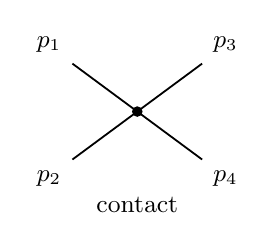
\begin{tikzpicture}[x=.58cm,y=.58cm,baseline=-.55ex,
                    line/.style={line width=.65pt},
                    vertex/.style={circle,fill,inner sep=1.35pt},
                    every node/.style={font=\small}]
 \path (-2.05,-2.35) (2.05,1.45);
 \coordinate (c) at (0,0);
 \draw[line] (-1.42,1.05)--(c)--(1.42,1.05);
 \draw[line] (-1.42,-1.05)--(c)--(1.42,-1.05);
 \node[vertex] at (c) {};
 \node[anchor=south east] at (-1.45,1.08) {\(p_1\)};
 \node[anchor=north east] at (-1.45,-1.08) {\(p_2\)};
 \node[anchor=south west] at (1.45,1.08) {\(p_3\)};
 \node[anchor=north west] at (1.45,-1.08) {\(p_4\)};
 \node at (0,-2.05) {contact};
\end{tikzpicture}
\quad
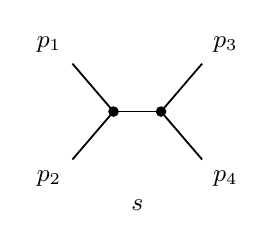
\begin{tikzpicture}[x=.58cm,y=.58cm,baseline=-.55ex,
                    line/.style={line width=.65pt},
                    vertex/.style={circle,fill,inner sep=1.35pt},
                    every node/.style={font=\small}]
 \path (-2.05,-2.35) (2.05,1.45);
 \coordinate (a) at (-.52,0); \coordinate (b) at (.52,0);
 \draw[line] (-1.42,1.05)--(a)--(-1.42,-1.05);
 \draw[line] (a)--(b);
 \draw[line] (1.42,1.05)--(b)--(1.42,-1.05);
 \node[vertex] at (a) {}; \node[vertex] at (b) {};
 \node[anchor=south east] at (-1.45,1.08) {\(p_1\)};
 \node[anchor=north east] at (-1.45,-1.08) {\(p_2\)};
 \node[anchor=south west] at (1.45,1.08) {\(p_3\)};
 \node[anchor=north west] at (1.45,-1.08) {\(p_4\)};
 \node at (0,-2.05) {\(s\)};
\end{tikzpicture}
\quad
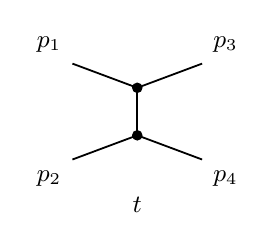
\begin{tikzpicture}[x=.58cm,y=.58cm,baseline=-.55ex,
                    line/.style={line width=.65pt},
                    vertex/.style={circle,fill,inner sep=1.35pt},
                    every node/.style={font=\small}]
 \path (-2.05,-2.35) (2.05,1.45);
 \coordinate (a) at (0,.52); \coordinate (b) at (0,-.52);
 \draw[line] (-1.42,1.05)--(a)--(1.42,1.05);
 \draw[line] (a)--(b);
 \draw[line] (-1.42,-1.05)--(b)--(1.42,-1.05);
 \node[vertex] at (a) {}; \node[vertex] at (b) {};
 \node[anchor=south east] at (-1.45,1.08) {\(p_1\)};
 \node[anchor=north east] at (-1.45,-1.08) {\(p_2\)};
 \node[anchor=south west] at (1.45,1.08) {\(p_3\)};
 \node[anchor=north west] at (1.45,-1.08) {\(p_4\)};
 \node at (0,-2.05) {\(t\)};
\end{tikzpicture}
\quad
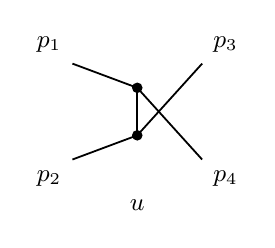
\begin{tikzpicture}[x=.58cm,y=.58cm,baseline=-.55ex,
                    line/.style={line width=.65pt},
                    vertex/.style={circle,fill,inner sep=1.35pt},
                    every node/.style={font=\small}]
 \path (-2.05,-2.35) (2.05,1.45);
 \coordinate (a) at (0,.52); \coordinate (b) at (0,-.52);
 \draw[line] (-1.42,1.05)--(a)--(1.42,-1.05);
 \draw[line] (a)--(b);
 \draw[line] (-1.42,-1.05)--(b)--(1.42,1.05);
 \node[vertex] at (a) {}; \node[vertex] at (b) {};
 \node[anchor=south east] at (-1.45,1.08) {\(p_1\)};
 \node[anchor=north east] at (-1.45,-1.08) {\(p_2\)};
 \node[anchor=south west] at (1.45,1.08) {\(p_3\)};
 \node[anchor=north west] at (1.45,-1.08) {\(p_4\)};
 \node at (0,-2.05) {\(u\)};
\end{tikzpicture}.
\]
\item
Let \(p_1,p_2,p_3,p_4\) denote all-incoming external momenta.  Then
\[
 \sum_{i=1}^4p_i=0,
 \qquad p_i^2=-m^2.
\]
For
\(q_s=p_1+p_2\), \(q_t=p_1+p_3\), and
\(q_u=p_1+p_4\), these relations imply
\[
 q_s^2+q_t^2+q_u^2=-4m^2.
\]
At either end of an exchange line, the two external inverse
propagators vanish on shell, so the cubic rule reduces to
\(-2i\lambda(q_x^2+m^2)\).  The contribution of one channel is
therefore
\[
 \bigl[-2i\lambda(q_x^2+m^2)\bigr]^2
 \frac{-i}{q_x^2+m^2-i0}
 =4i\lambda^2(q_x^2+m^2).
\]
Summing the three exchange graphs gives
\[
 \mathcal A_{\rm exch}
 =4i\lambda^2(q_s^2+q_t^2+q_u^2+3m^2)
 =-4i\lambda^2m^2.
\]
The on-shell contact rule is
\[
 \mathcal A_{\rm contact}
 =-4i\lambda^2(-4m^2+3m^2)
 =4i\lambda^2m^2.
\]
Consequently
\[
 \boxed{\mathcal A_{\rm connected}
 =\mathcal A_{\rm contact}+\mathcal A_{\rm exch}=0}.
\]
The original \(\Phi\) theory is free, so this cancellation is exactly
what invariance of the on-shell \(S\)-matrix under a local invertible
field redefinition requires, even though the redefined Lagrangian
contains nonzero off-shell vertices.
\end{enumerate}

\SupplementarySolution{9}{Field Redefinitions, External Poles, and Order Bookkeeping}
\begin{enumerate}
\item
Seek
\[
 \phi=\phi'+\epsilon A\phi'^2+\epsilon^2B\phi'^3+O(\epsilon^3).
\]
Substitution into
\(\phi'=\phi+\epsilon\phi^2+\epsilon^2a\phi^3\) gives
\[
 0=\epsilon(A+1)\phi'^2
 +\epsilon^2(B+2A+a)\phi'^3.
\]
Thus \(A=-1\), \(B=2-a\), and
\[
 \phi=\phi'-\epsilon\phi'^2
       +\epsilon^2(2-a)\phi'^3+O(\epsilon^3).
\]
Local admissibility requires a nonzero functional Jacobian.  Pointwise,
\(\partial\phi'/\partial\phi
=1+2\epsilon\phi+3a\epsilon^2\phi^2\ne0\) in the field region under
consideration.  Perturbatively this holds near the identity.
\item
Near the physical one-particle pole, the Fourier transform of the new
two-point function has the spectral form
\[
 \widetilde G_{\phi'}(p)
 =\frac{Z'}{p^2+m_{\rm phys}^2-i0}
  +\text{terms regular at the pole}.
\]
The composite term \(\epsilon\phi^2\) changes the overlap
\(\bra{\Omega}\phi'(0)\ket{p}\), and hence changes \(Z'\), but it cannot
move the pole because the mass is a property of the Hamiltonian
spectrum.  Amputation multiplies by the inverse pole and divides each
external leg by \(\sqrt{Z'}\).  The overlap change then cancels, leaving
the same on-shell scattering observable provided \(Z'\ne0\).  Off-shell
correlators need not agree.
\item
For
\(\phi\mapsto\phi+\epsilon F\), Taylor expansion of the action gives
\[
 S[\phi+\epsilon F]
 =S[\phi]+\epsilon\int F\frac{\delta S}{\delta\phi}
 +\frac{\epsilon^2}{2}\int d^4x\,d^4y\,
 F(x)\frac{\delta^2S}{\delta\phi(x)\delta\phi(y)}F(y)+\cdots .
\]
The linear term can cancel a chosen dimension-six equation-of-motion
operator.  The quadratic term contains two powers of the suppressed
coefficient and therefore contributes at the dimension-eight order in
the same power counting.  Omitting it is consistent in a calculation
truncated at first order in \(\epsilon\), but not in a second-order
calculation, where it is required for equivalence.
\end{enumerate}

\SupplementarySolution{10}{Geometry, Hamiltonian, and Current of the \(O(N)\) Sigma Model}
\begin{enumerate}
\item
Write
\[
 n^A=(\pi^a,\sigma),\qquad
 \sigma=\sqrt{1-\boldsymbol\pi^2}.
\]
Then
\[
 \partial_\mu\sigma
 =-\frac{\pi_a\partial_\mu\pi^a}
         {\sqrt{1-\boldsymbol\pi^2}},
\]
and hence
\[
 \partial_\mu n^A\partial^\mu n^A
 =g_{ab}(\pi)\partial_\mu\pi^a\partial^\mu\pi^b,
\qquad
 g_{ab}=\delta_{ab}
 +\frac{\pi_a\pi_b}{1-\boldsymbol\pi^2}.
\]
The apparent interaction is therefore the metric induced on the unit
sphere.  The coordinate patch fails at
\(\boldsymbol\pi^2=1\), where the eliminated component \(\sigma\)
vanishes, even though the sphere itself is regular.
\item
The rank-one inverse is
\[
 g^{ab}=\delta^{ab}-\pi^a\pi^b,
\qquad g_{ac}g^{cb}=\delta_a{}^b .
\]
For
\[
 \mathcal L=-\frac1{2e^2}g_{ab}
 \partial_\mu\pi^a\partial^\mu\pi^b,
\]
the canonical momentum is
\[
 p_a=\frac1{e^2}g_{ab}\dot\pi^b .
\]
Solving for the velocity and performing the Legendre transform gives
\[
 \mathcal H
 =\frac{e^2}{2}p_ag^{ab}p_b
 +\frac1{2e^2}g_{ab}
 \boldsymbol\nabla\pi^a\cdot\boldsymbol\nabla\pi^b .
\]
The inverse target metric necessarily appears in the momentum term,
just as in the general nonlinear sigma-model Hamiltonian.
\item
For a rotation in the \(AB\)-plane,
\(\delta n^A=\epsilon n^B\) and
\(\delta n^B=-\epsilon n^A\).  Noether's theorem gives, up to the
orientation convention,
\[
 j^\mu_{AB}=\frac1{e^2}
 \left(n^A\partial^\mu n^B-n^B\partial^\mu n^A\right).
\]
The constrained equation has the form
\[
 \Box n^A=\lambda(x)n^A,
\]
because the force normal to the sphere is supplied by a Lagrange
multiplier.  Therefore
\[
 \partial_\mu j^\mu_{AB}
 =\frac1{e^2}(n^A\Box n^B-n^B\Box n^A)=0.
\]
The unknown multiplier cancels, so conservation follows without solving
for it.
\end{enumerate}

\SupplementarySolution{11}{Quantization and Charge of a Complex Scalar Field}
\begin{enumerate}
\item
At equal time, insert the mode expansion into
\([\Phi(\mathbf x),\dot\Phi^\dagger(\mathbf y)]\).  The terms containing
\(a\) and \(a^\dagger\) and those containing \(b^\dagger\) and \(b\)
must reproduce the Fourier representation of the delta function.  One
finds two independent oscillator algebras,
\[
 \boxed{
 [a_{\mathbf p},a_{\mathbf q}^\dagger]
 =[b_{\mathbf p},b_{\mathbf q}^\dagger]
 =(2\pi)^{D-1}\delta^{D-1}(\mathbf p-\mathbf q),}
\]
with
\[
 [a_{\mathbf p},a_{\mathbf q}]
 =[b_{\mathbf p},b_{\mathbf q}]
 =[a_{\mathbf p},b_{\mathbf q}]
 =[a_{\mathbf p},b_{\mathbf q}^\dagger]=0,
\]
and the Hermitian conjugates of these relations.  In particular the
particle and antiparticle oscillators are unrelated, as required for a
complex field.
\item
The Hamiltonian density is
\[
 \mathcal H
 =\dot\Phi^\dagger\dot\Phi
 +\boldsymbol\nabla\Phi^\dagger\cdot\boldsymbol\nabla\Phi
 +m^2\Phi^\dagger\Phi.
\]
The spatial integral kills the mixed terms; on the mass shell
\(E_{\mathbf p}^2=\mathbf p^2+m^2\).  Hence
\[
 H=\int\frac{d^{D-1}\mathbf p}{(2\pi)^{D-1}}
 E_{\mathbf p}
 \left(a_{\mathbf p}^\dagger a_{\mathbf p}
 +b_{\mathbf p}b_{\mathbf p}^\dagger\right).
\]
Reordering the second term gives
\[
 \boxed{
 H=\int\frac{d^{D-1}\mathbf p}{(2\pi)^{D-1}}
 E_{\mathbf p}
 \left(a_{\mathbf p}^\dagger a_{\mathbf p}
 +b_{\mathbf p}^\dagger b_{\mathbf p}\right)
 +E_{\rm vac},}
\]
where
\(E_{\rm vac}=\delta^{D-1}(0)\int d^{D-1}\mathbf p\,E_{\mathbf p}\)
in the displayed continuum normalization.  Normal ordering removes this
state-independent constant.
\item
Since \(\partial^0=-\partial_0\), the supplied current gives
\[
 Q=i\int d^{D-1}\mathbf x\left(
 \dot\Phi^\dagger\Phi-\Phi^\dagger\dot\Phi\right).
\]
Substitution of the modes yields, after normal ordering,
\[
 \boxed{
 Q=\int\frac{d^{D-1}\mathbf p}{(2\pi)^{D-1}}
 \left(b_{\mathbf p}^\dagger b_{\mathbf p}
 -a_{\mathbf p}^\dagger a_{\mathbf p}\right).}
\]
Therefore
\[
 Q,a_{\mathbf p}^\dagger\ket{\Omega}
 =-a_{\mathbf p}^\dagger\ket{\Omega},
 \qquad
 Q,b_{\mathbf p}^\dagger\ket{\Omega}
 =+b_{\mathbf p}^\dagger\ket{\Omega}.
\]
Thus the two equal-mass species have opposite conserved charges.  Which
one is called the particle is a convention tied to the sign chosen for
the current; either way, one species is the antiparticle of the other.
\end{enumerate}
\end{enumerate}
